

\section{Введение}
Одним из фундаментальных принципов классической механики является принцип эквивалентности масс, утверждающий, что инертная и гравитационная массы тела равны. Этот принцип лежит в основе общей теории относительности Эйнштейна, но его истоки восходят к экспериментальным и теоретическим исследованиям Галилея, опровергшим представления Аристотеля о зависимости скорости падения тел от их массы.

\parАристотель полагал, что более массивные тела падают быстрее, однако Галилей показал, что это приводит к логическому противоречию. 
\parДанная лабораторная работа направлена на экспериментальную проверку принципа эквивалентности масс путём сравнения ускорения свободного падения для тел различной плотности.




\subsection{Задачи работы}

Таким образом, задачами данной работы являются:
\begin{enumerate}
    \item Проверить принцип эквивалентности масс.
    \item Измерить ускорение свободного падения тел.
    \item Познакомиться с методом измерения интервалов времени между импульсами
частотомером – хронометром Ч3-32.
    \item Определение погрешности косвенных измерений.
\end{enumerate}




\section{Основная часть}

\subsection{Теоретическая часть}
Инертную массу тела можно определить, измерив ускорение $\vec{a}$, которое испытывает тело под действием известной силы $\vec{F}$:
\begin{equation}
    M_{ин}=\frac{|\vec{F}|}{|\vec{a}|}
\end{equation}
\parГравитационную  массу тела можно определить по следующей формуле:
\begin{equation}
 M_{p} = \frac{F r^{2}}{\gamma M_{3}},
\end{equation}
где $M_{з}$ - масса Земли, $\gamma$ - гравитационная постоянная, r - расстояние между центром Земли и телом.
\parСовременные эксперименты с большой точностью подтверждают равенство инертной и гравитационной масс. 
\parЛокально невозможно отличить однородное гравитационное поле от равноускоренного движения системы отсчёта. Иными словами, в достаточно малой области пространства-времени все физические процессы протекают одинаково в двух случаях:
\begin{enumerate}
    \item  В инерциальной системе отсчёта в отсутствие гравитации.
    \item  В неинерциальной системе отсчёта, движущейся с постоянным ускорением $g$, или в покоящейся системе отсчёта в присутствии однородного гравитационного поля с напряжённостью $-g$.
\end{enumerate}
\par Представим доказательство этого утверждения:



\parУравнение движения произвольной системы частиц в инерциальной системе координат при наличии однородного гравитационного поля имеют следующий вид:
\begin{equation}
\label{eq3}
m_k \frac{d^{\, 2}\vec{x}_k}{dt^{\, 2}} = m_k\vec{g} + \sum_{\substack{i=1 \\ i\neq k}}^{N}  \vec{F}(\vec{x}_k - \vec{x}_i)\,,
\end{equation}
где $\vec{F}(\vec{x}_k - \vec{x}_i)$ - внутренние силы между частицами системы.
\par Произведя замену переменной x, перейдём в систему координат, осуществляющую движение с ускорением $g$ относительно исходной:
\begin{equation}
\label{eq4}
\vec{x}' = \vec{x} - \frac{\vec{g}t^2}{2}, \quad t' = t,
\end{equation}
подставив в равенство (\ref{eq:eq3}) получим:
\begin{equation}
\label{eq5}
m_k \frac{d^{\, 2}\vec{x}_k}{dt^{\, 2}} =  \sum_{\substack{i=1 \\ i\neq k}}^{N}  \vec{F}(\vec{x}_k - \vec{x}_i)
\end{equation}
\parУравнение (\ref{eq:eq5}) совпадает с уравнением (\ref{eq:eq3}), если $g$=0. Становится понятно, что $\vec{g}$ не зависит от $t$ и $\vec{x}$. Утверждение доказано.

\subsection{Эксперимент}
Если верен принцип эквивалентности масс, то время свободного падения тел с разной массой (при прочих равных условиях) должно быть одинаковым. Цель данной лабораторной работы – экспериментально проверить это утверждение.
\begin{figure}[H]
\centering
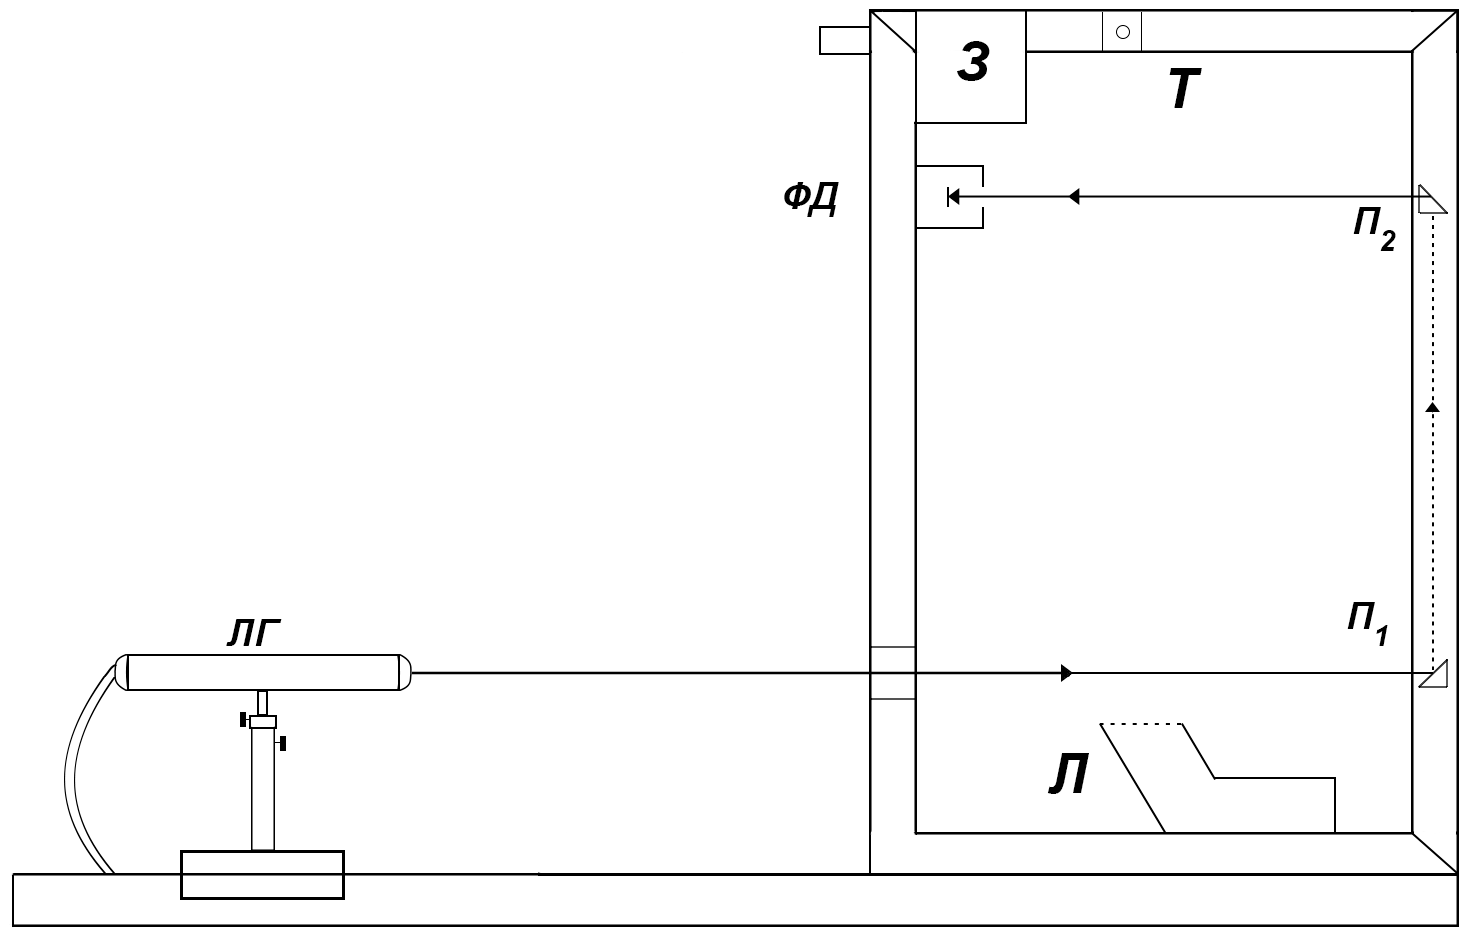
\includegraphics[width=0.8\textwidth]{Схема установки.png}
\caption{Схема установки}
\label{fig:1}
\end{figure}
\begin{figure}[H]
\centering
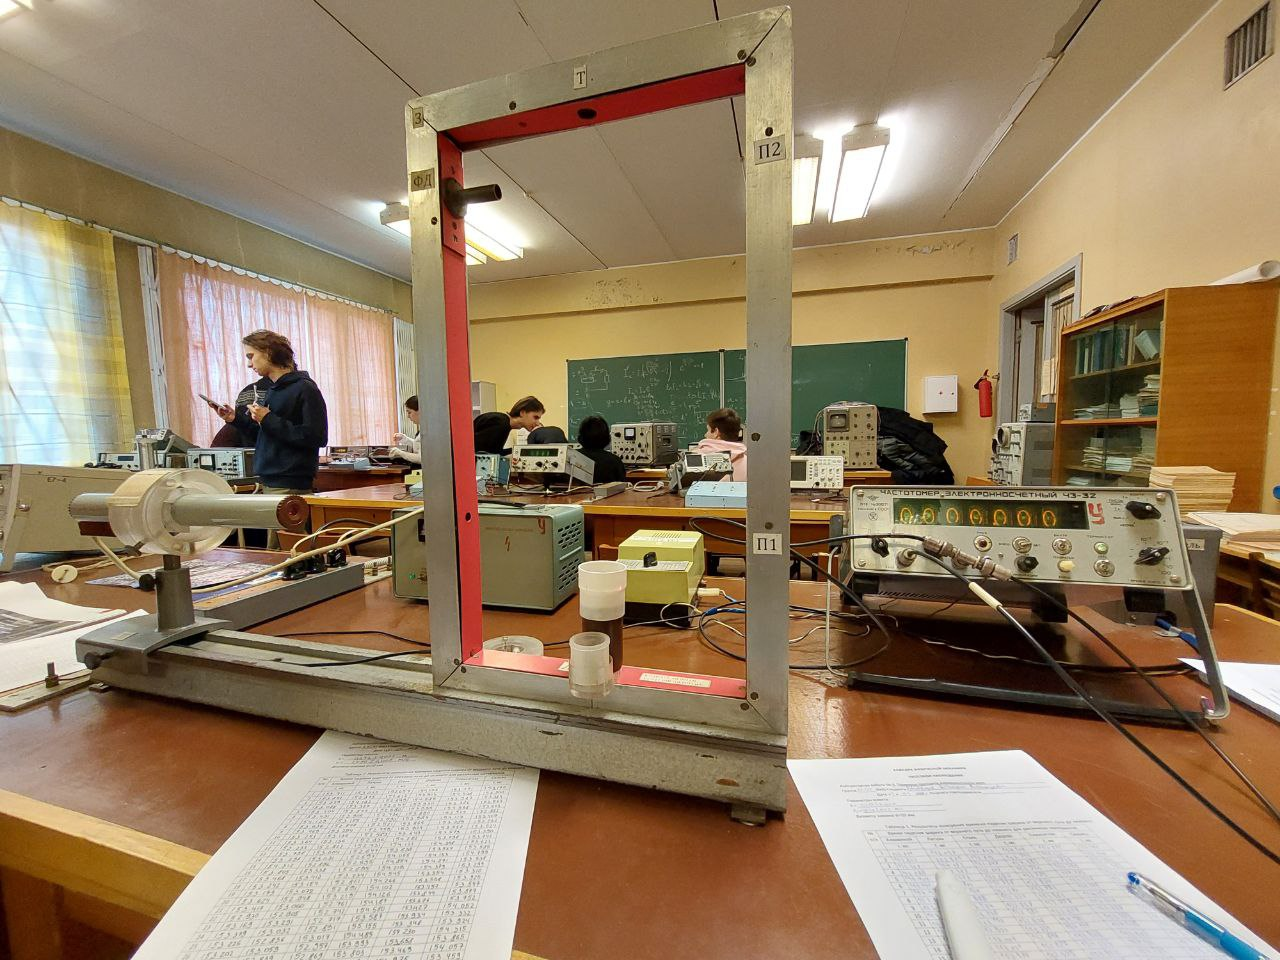
\includegraphics[width=0.8\textwidth]{Фотография установки.jpg}
\caption{Фотография установки}
\label{fig:2}
\end{figure}
\parСхема установки приведена на рисунке \ref{fig:1}. Луч от квантового генератора \textbf{ЛГ} направляется на призму полного внутреннего отражения \textbf{П$_1$}, от нее на призму \textbf{П$_2$}, а затем на фотодиод \textbf{ФД}. При отодвигании заслонки З шарик, находящийся в трубке \textbf{Т}, падает в лузу \textbf{Л} и пересекает два световых луча, расстояние между которыми равно h . Когда шарик пересекает верхний луч, фотодиод \textbf{ФД} вырабатывает импульс, который усилившись в усилителе, подается на вход частотомера Ч3-32 и запускает его. При пересечении шариком нижнего луча импульс от фотодиода останавливает счет частотомера. Интервал времени между двумя импульсами, регистрируемый частотомером, равен времени пролета t шарика от верхнего луча до нижнего. Усилитель питается от источника УПУ-1У4.
\\
\parМасса вещества была посчитана по формуле:
\begin{equation}
\label{eq:6}
    m=\frac{\rho}{V},  V=\frac{4\cdot\pi\cdot(\frac{d}{2})^3}{3},
\end{equation}
где $\rho$ - плотность вещества, d - диаметр шара.
\begin{center}
\begin{table}[H]
\centering
\caption{Таблица веществ}
\label{table:1}
\begin{tabular}{|c|c|c|c|c|}
\hline
{} № п/п & Вещество & Плотность & Диаметр & Масса \\
\hline
{} &  & \( 10^3 \, \frac{\text{кг}}{\text{м}^3} \) & \( 10^{-3} \, \text{м} \) & \( 10^{-6} \, \text{кг} \) \\
\hline
1 & Дерево & 0,7 & 1 & 0.4  \\
2 & Плексиглас & 1,18 & 1 & 0.6  \\
3 & Алюминий & 2,79 & 1 & 1  \\
4 & Сталь & 7,9 & 1 &  4 \\
5 & Латунь & 8,5 & 1 & 4  \\
6 & Свинец & 11,34 & 1 &  6 \\
\hline
\end{tabular}
\end{table}
\end{center}


\begin{center}
\begin{table}[H]
\centering
\caption{Результаты измерения времени падения шарика от верхнего луча до нижнего}

\label{table:t1}
\begin{tabular}{|c|c|c|c|c|c|c|}
\hline

№ п.п. &Алюминий&Латунь&Сталь&Дерево&Плексиглас&Свинец\\
\hline
{}&t, мс&t, мс&t, мс&t, мс&t, мс&t, мс\\
\hline
1 & 153.711 & 153.039 & 152.657 & 154.106 & 153.791 & 153.170 \\
2 & 153.852 & 152.875 & 152.612 & 153.913 & 154.508 & 152.900 \\
3 & 153.329 & 154.192 & 152.649 & 154.585 & 153.987 & 153.384 \\
4 & 153.088 & 153.367 & 152.647 & 153.930 & 153.386 & 152.563 \\
5 & 153.404 & 153.577 & 152.680 & 153.995 & 153.998 & 152.203\\
6 & 153.431 & 153.905 & 152.736 & 153.890 & 153.525 & 152.881 \\
7 & 154.129 & 153.155 & 152.590 & 153.983 & 154.117 & 153.407 \\
8 & 153.636 & 152.878 & 152.521 & 153.865 & 153.289 & 152.562 \\
9 & 153.469 & 153.254 & 152.759 & 153.927 & 153.557 & 153.524 \\
10 & 153.253 & 153.136 & 152.583 & 153.647 & 153.579 & 153.390 \\
\hline
\end{tabular}
\end{table}
\end{center}
\begin{center}
\begin{table}[H]
\centering
\caption{Результаты измерения времени падения шарика от верхнего луча до нижнего}

\label{table:t1}
\begin{tabular}{|c|c|c|c|c|c|c|}
\hline

№ п.п. &Алюминий&Латунь&Сталь&Дерево&Плексиглас&Свинец\\
\hline
{}&t, мс&t, мс&t, мс&t, мс&t, мс&t, мс\\
\hline
11 & 153.364 & 153.136 & 152.836 & 154.282 & 153.798 & 153.742 \\
12 & 153.233 & 152.822 & 152.731 & 154.121 & 154.348 & 153.622 \\
13 & 153.798 & 153.004 & 152.647 & 153.838 & 153.567 & 153.585 \\
14 & 153.298 & 153.031 & 152.697 & 154.055 & 154.133 & 154.799 \\
15 & 154.312 & 152.896 & 152.595 & 154.854 & 154.271 & 153.538 \\
16 & 153.805 & 153.338 & 152.695 & 154.219 & 154.379 & 153.299 \\
17 & 153.468 & 153.412 & 153.234 & 154.545 & 153.354 & 153.310 \\
18 & 153.242 & 153.154 & 152.861 & 154.266 & 153.508 & 153.925 \\
19 & 153.173 & 153.072 & 153.691 & 154.102 & 153.457 & 153.547 \\
20 & 153.624 & 152.948 & 153.219 & 154.126 & 153.844 & 153.877 \\
21 & 153.417 & 153.060 & 152.761 & 154.187 & 153.676 & 153.752 \\
22 & 152.930 & 152.905 & 152.742 & 154.580 & 153.427 & 154.052 \\
23 & 153.169 & 153.291 & 152.717 & 153.587 & 153.934 & 153.332 \\
24 & 153.379 & 153.032 & 152.891 & 155.155 & 153.348 & 153.924 \\
25 & 153.226 & 152.836 & 153.017 & 154.485 & 154.230 & 154.315 \\
26 & 153.202 & 153.059 & 152.954 & 153.993 & 153.658 & 153.865 \\
27 & 153.246 & 152.839 & 152.869 & 153.803 & 153.469 & 154.057 \\
28 & 152.514 & 152.999 & 152.854 & 154.108 & 153.975 & 153.459 \\
29 & 152.914 & 153.312 & 152.827 & 154.328 & 153.549 & 153.781 \\
30 & 153.729 & 153.089 & 152.797 & 153.985 & 153.444 & 154.085 \\
\hline
$\overline{t}$ & 153.412 &  153.154 & 152.802 & 154.149& 153.770 & 153.528 \\
\hline
\end{tabular}
\end{table}
\end{center}
\parФормула для нахождение погрешности времени пролёта шариков:
\begin{equation}
    \label{eq:7}
    \Delta\overline{t}=\frac{\sqrt{\frac{\Sigma(t_i-\overline{t})^2}{{n-1}}}}{\sqrt{n}}
\end{equation}
\begin{center}
\begin{table}[H]
\centering
\caption{Погрешность времени пролета шариков, $\Delta$t}
\label{table:1}
\begin{tabular}{|c|c|}
\hline
{} Вещество & $\Delta$t, мс \\
\hline
Алюминий & 0.0664068\\
Латунь &0.0564740  \\
Сталь &0.0434828  \\
Дерево      &0.0627690    \\
Плексиглас     &0.0643578  \\
Свинец     &0.0993112   \\
\hline
\end{tabular}
\end{table}
\end{center}
\parУравнение движения при свободном падении имеет следующий вид:
\begin{equation}
    \label{eq:8}
    h= v_0 t + \frac{g t^2}{2} 
\end{equation}
\parСледовательно,
\begin{equation}
    \label{eq:9}
    g= \frac{2(h - v_0 \overline{t})}{\overline{t}^2} 
\end{equation}
\parХарактеристики установки \ref{fig:1}: $h=(0.272\pm0.001)$ м, $v_0=(1.050\pm0.005)$ м/с.

\begin{center}
\begin{table}[H]
\centering
\caption{Ускорение свободного падения, $g$}
\label{table:4}
\begin{tabular}{|c|c|c|}
\hline
{} № п/п & Вещество & $g$, м/с$^2$ \\
\hline
1 & Алюминий     & 9.43 \\
2 & Латунь & 9.48\\
3 & Сталь   &9.56 \\
4 & Дерево       &9.27 \\
5 & Плексиглас     &9.35 \\
6 & Свинец     &9.40 \\
\hline
\end{tabular}
\end{table}
\end{center}
\parПогрешность свободного ускорения ищется по формуле погрешности косвенных измерений, в предположении, что $g$ зависит от $t$, $h$, $v_0$:
\begin{equation}
    \label{eq:10}
   \Delta g = \sqrt{
    \frac{1}{9} \left(\frac{\partial g}{\partial h}\right)^2 \Delta{h}^2 +
    \frac{1}{9} \left(\frac{\partial g}{\partial v_0}\right)^2 \Delta{v_0}^2 +
    \left(\frac{\partial g}{\partial t}\right)^2 \Delta{\overline{t}}^2}
\end{equation}
После вычислений формула принимает вид:
\begin{equation}
    \label{eq:11}
   \Delta g = \sqrt{
    \frac{1}{9} \left(\frac{2}{\overline{t}^2}\right)^2 \Delta{h}^2 +
    \frac{1}{9} \left(\frac{-2}{\overline{t}}\right)^2 \Delta{v_0}^2 +
    \left(\frac{2(v_0\overline{t}-2h)}{\overline{t}^3}\right)^2 \Delta{\overline{t}}^2}
\end{equation}
\begin{center}
\begin{table}[H]
\centering
\caption{Погрешность ускорения свободного падения, $\Delta g$}
\label{table:4}
\begin{tabular}{|c|c|c|}
\hline
{} № п/п & Вещество & $\Delta g$, м/с$^2$ \\
\hline
1 & Алюминий     & 0.03 \\
2 & Латунь & 0.03\\
3 & Сталь   &0.02 \\
4 & Дерево       &0.03 \\
5 & Плексиглас     &0.03 \\
6 & Свинец     &0.03 \\
\hline
\end{tabular}
\end{table}
\end{center}





\subsubsection{Исходный код}
Исходный код состоит из двух решений: "Mass", "Program".

\begin{center}\parНиже представлено описание кода решения "Mass":\end{center}
\parФункция inputdata() осуществляет ввод исходных данных из файла \\"InputData.csv"\verb||
и сохранения их в массив arr1, arr2.
\parФункция mass() вычисляет значение масс шариков по формуле (\ref{eq:6}).
\parФункция outputdata() записывает вычисленные массы в файл "OutputData.csv".

\begin{center}\parНиже представлено описание кода решения "Program":\end{center}
\parФункция inputdata() осуществляет ввод исходных данных из файла \\"InputData.csv"\verb||
и записывает в двумерный массив arr.
\parФункция calculate\underline{ }average() вычисляет среднее значение пролёта шарика для каждого из шести образцов.
\parФункция time\underline{ }error() вычисляет погрешность пролёта шарика для каждого из шести образцов по формуле по формуле (\ref{eq:7}).
\parФункция  acceleration() вычисляет ускорение свободного падения для шести шариков по формуле (\ref{eq:9}).
\parФункция gerror\underline{ }calc() вычисляет погрешность ускорения свободного падения по формуле (\ref{eq:11}).
\parФункция outputdata() записывает вычисленные массы в файл "OutputData.csv".

\subsubsection{Анализ ошибок}
\parПри измерении ускорения свободного падения возникают систематические ошибки, которые искажают результаты. Они приводят к смещению результата в одну сторону (завышению или занижению). В отличие от случайных ошибок, их нельзя устранить простым увеличением числа измерений, но можно выявить и скорректировать.
\parПри движении тела в воздухе на него действует сила сопротивления среды (воздуха), которая замедляет падение и искажает результаты измерений. Эта сила зависит от скорости, формы и площади поверхности тела, а также от свойств воздуха (плотности, вязкости). Сопротивление воздуха приводит к занижению измеряемого значения $g$.

\section{Выводы}
В ходе лабораторной работы были проведены измерения времени пролёта шариков разной массы на расстояние $h$ с начальной скоростью $v_0$. Кроме того, были высчитаны погрешность времени и погрешность свободного ускорения. Проведён анализ систематических погрешностей и их источников.


\begin{thebibliography}{9}

%ссылка на репозиторий с исходныим кодом отчета и всех расчетных программ 
\bibitem{repo}
\url{https://github.com/st117207/Workshop4}  (дата обращения: 24.04.2025) 


\end{thebibliography}

